% Requires running Bibtex

\documentclass[%
reprint,
amsmath,amssymb,
aps,
floatfix
]{revtex4-2}

\usepackage{graphicx}% Include figure files
\usepackage{dcolumn}% Align table columns on decimal point
\usepackage{bm}% bold math
\usepackage{hyperref}% add hypertext capabilities
\usepackage[font=scriptsize,labelfont=bf, justification=justified]{caption}% change fontsize in captions
\usepackage{float}
\usepackage{booktabs}% cool table style
\hypersetup{
	colorlinks=true,       % false: boxed links; true: colored links
	linkcolor=black,        % color of internal links
	citecolor=black,        % color of links to bibliography
	filecolor=black,     % color of file links
	urlcolor=black         
}

\usepackage{listings}

%\usepackage{bibspacing}
%\setlength{\bibitemsep}{.5\baselineskip plus .05\baselineskip minus .05\baselineskip}


\begin{document}
	
	\preprint{APS/123-QED}
	
	\title{PHYC30170 Physics with Astronomy and Space Science Lab 1;\\Electronics}
	
	\author{Daragh Hollman}
	\email{daragh.hollman@ucdconnect.ie}
	
	\date{\today}
	
	\maketitle
	
	\section{Introduction}
		This report features 8 exercises of the 31 included in the 3rd Year Electronics Laboratory manual \cite{manual}. The exercises make use of a combination of simulations carried out on a computer and actual physically creating the circuits to measure them. Many areas of electronics were covered including RC circuits, diodes, transistors, op-amps, and DACs.
	
	\section{Exercise 5: RC Circuits}
		\subsection{Theory}
		Exercise 5 involves the construction and measurement of a RC circuit. An RC circuit is one which consists of a resistor and capacitor. The capacitor stores charge and the resistor controls the rate at which it discharges \cite{pumplin}. This time dependent discharge is an exponential decay given by the following equation:
		\begin{equation}
			V_\text{out} = V_\text{in} \exp{\left(\frac{-t}{RC}\right)}
			\label{eq:expDecay}
		\end{equation}where $V_\text{in}$ is the input voltage and $V_\text{out}$ is the voltage output measured by the voltmeter in figure \ref{fig:sampleRC}. $R$ and $C$ are simply the resistance and capacitance respectively. The factor $1/RC$ is defined as the decay constant which solely determines the rate of decay \cite{manual}.
		
		\begin{figure}
			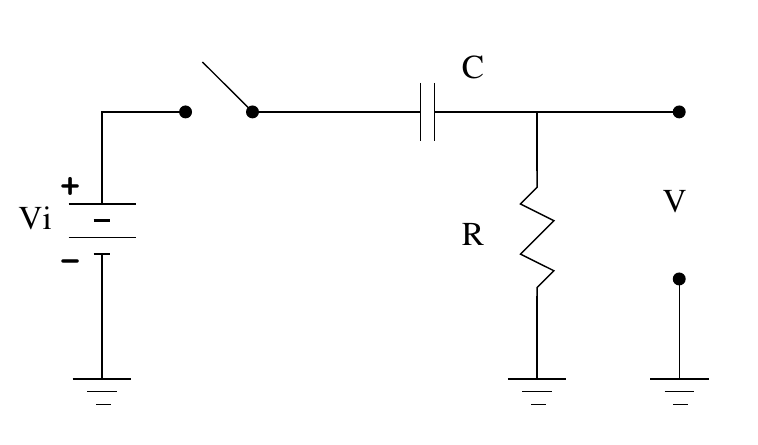
\includegraphics[width=0.85\columnwidth]{sampleRC.png}
			\caption{\label{fig:sampleRC}A sample RC circuit as described in the lab manual \cite{manual}.}
		\end{figure}
	
		\subsection{Methodology}
		The RC circuit depicted in figure \ref{fig:sampleRC} was constructed in DesignSoft's TINA \cite{TINA}, a circuit simulator. This construction is shown in figure \ref{fig:ex5Circuit}. A virtual oscilloscope was used in place of a voltmeter to measure the signal as a function of time. The component values of the capacitor and resistor were chosen as directed by the exercise and a square wave of frequency $20 \,\text{Hz}$ with peak to peak amplitude of $5\,\text{V}$ was used as the input. The circuit was simulated and the signal was recorded. The circuit was then constructed physically on a breadboard and the same measurement was made using an oscilloscope. The signals of the simulation, the measurement, and the analytical solution were then compared and the decay constants determined.
		
		\begin{figure}
			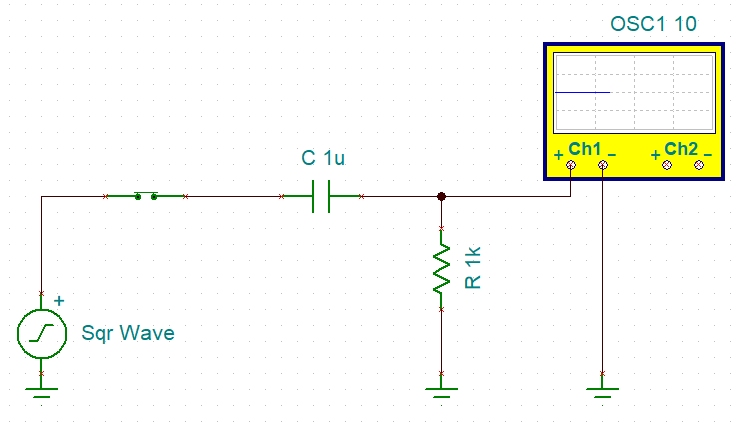
\includegraphics[width=0.85\columnwidth]{circuit_ex5.png}
			\caption{\label{fig:ex5Circuit}The circuit construction created in TINA for simulation.}
		\end{figure}
		
		\subsection{Results \& Analysis}
		The measured data from the breadboard were plotted in figure \ref{fig:ex5Results} along with the analytical solution calculated using equation \ref{eq:expDecay}. The decay constant of the analytical solution was calculated from the values of the resistor and the capacitor however, the decay constants for the measured data and simulation data were determined using least squares fitting of the signal. The decay constants for each method were recorded in table \ref{tab:decayConstants} along with their uncertainty which was determined by the square root of the diagonal elements of the covariance matrix. 
		
		\begin{table}[]
			\resizebox{0.85\columnwidth}{!}{%
				\begin{tabular}{@{}lll@{}}
					\toprule
					Method     & Decay Constant ($s^{-1}$) & Uncertainty \\ \midrule
					Analytical & 1000                    & N/A         \\
					Simulation & 1012.884                 & $\mathcal{O}10^{-6}$           \\
					Measured   & 895.937                  & $\mathcal{O}10^{-6}$           \\ \bottomrule
				\end{tabular}%
			}
			\caption{Decay constants for exercise 5. The uncertainties were determined by the square root of the diagonal elements of the covariance matrix for least squares fitting}
			\label{tab:decayConstants}
		\end{table}
		
	
		\begin{figure}
			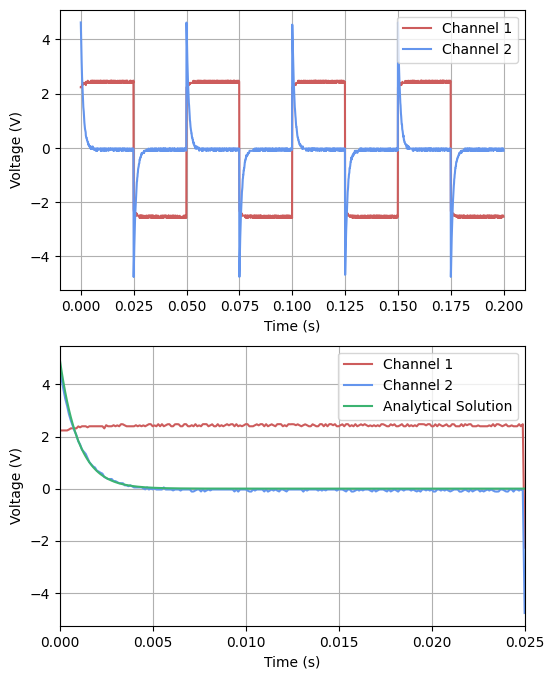
\includegraphics[width=0.85\columnwidth]{ex5_dualPlot.png}
			\caption{\label{fig:ex5Results}Input and output signals from the RC circuit in exercise 5. Channel 1 is the square wave driving the circuit whereas channel 2 is the output. The exponential decay response is clearly shown in the lower graph ($1\over2$ period) in comparison to the analytical solution.}
		\end{figure}
		\begin{figure}
			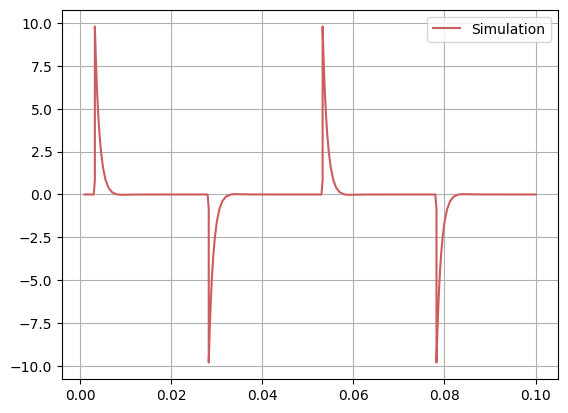
\includegraphics[width=0.85\columnwidth]{ex5_simPlot.png}
			\caption{\label{fig:ex5Sim}Simulation data generated by TINA, is exponential decay the same shape as the analytical and the measured.}
		\end{figure}
		\begin{figure}
			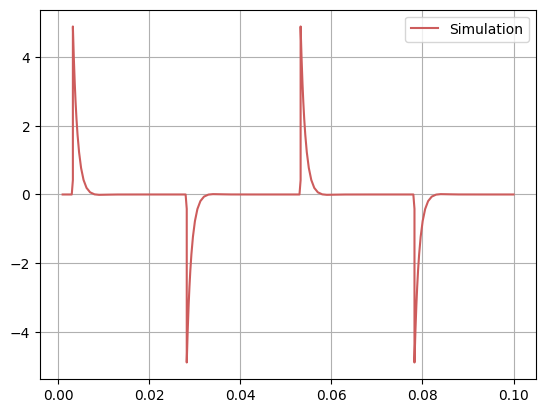
\includegraphics[width=0.85\columnwidth]{ex5_simPlotAdj.png}
			\caption{\label{fig:ex5SimAdj}The simulated data using peak to peak amplitude.}
		\end{figure}
	
		We notice that the amplitude of the simulation data is approximately twice that in the measured data. This is due to an inconsistency in the definition of amplitude, be it peak to peak amplitude or average to peak. We can still see clearly that the shape of the data matches what is expected and therefore dividing by two will yield the result under peak to peak amplitude. This is done explicitly in this exercise as shown in figures \ref{fig:ex5Sim} and \ref{fig:ex5SimAdj} however, for all further exercises where this applies - unless otherwise specified - this can be assumed to have been done.\\
		
		For consistency, in this report we shall use the term amplitude to refer to peak to peak amplitude as this is the definition used by the oscilloscope which was used to generate and measure signals for the majority of these exercises.
		
	\section{Exercise 7: RC Circuits and Frequency Filters}
		\subsection{Theory}
		Exercise 7 demonstrates how the same RC circuit as in exercise 5 can be used to make a high pass filter \cite{manual}. A high pass filter is a signal filter which allows higher frequencies to pass through unaffected but attenuates signals beyond a cut-off frequency. The combination of a resistor with a capacitor makes it possible to have voltage dividers dependent on frequency \cite{horowitz}. This frequency dependence arises from the impedance of the capacitor.
		\begin{equation}
			Z_C = -\frac{j}{\omega C}
			\label{eq:capacitor}
		\end{equation}where $j$ is the imaginary number $j=\sqrt{-1}$, $C$ is the capacitance, and $\omega$ is the angular frequency. For the circuit in figure \ref{fig:sampleRC}, by Ohm's law we have a current:
		\begin{equation}
			I = \frac{V_\text{in}}{Z_\text{total}} = \frac{V_\text{in}}{R - Z_C}
		\end{equation}and hence we can calculate the voltage across the resistor, $V_\text{out}$, by substitution and rationalisation of the denominator:
		\begin{equation}
			V_\text{out} = I R = V_\text{in}\frac{[R+(\frac{j}{\omega C})]R}{R^2 + (\frac{1}{\omega^2 C^2})}
		\end{equation}with a magnitude of:
		\begin{equation}
			V_\text{out} = V_\text{in}\frac{R}{\left[R^2 + \left(\frac{1}{\omega^2 C^2}\right)\right]^\frac{1}{2}} = V_\text{in} \frac{\omega R C}{\left[1 + \left(\omega RC\right)^2\right]^\frac{1}{2}}
			\label{eq:amplitude}
		\end{equation}this is derived in full by Horowitz and Hill \cite{horowitz} where they also determine the phase analyticity to be:
		\begin{equation}
			\phi = \arctan\left(\frac{-1}{\omega RC}\right)
			\label{eq:phase}
		\end{equation}which derives from the total impedance.	
	
		\subsection{Methodology}
		The aim of this exercise was to simulate and measure the amplitude and phase response of the RC circuit from exercise 5 when driven by a sin wave. The circuit was designed and created in TINA as shown in figure \ref{fig:ex7Circuit}. Note that this circuit is predominantly the same as in figure \ref{fig:ex5Circuit} in exercise 5, with the only difference being in the wave generated by the voltage generator. The circuit was simulated and the amplitude and phase response were recorded. The circuit was then constructed physically and the amplitude and phase response were measured using an oscilloscope for frequencies of 1 Hz, 10 Hz, 100 Hz, 1 kHz, 10 kHz, 100 kHz, and 1 MHz.
		
		\begin{figure}
			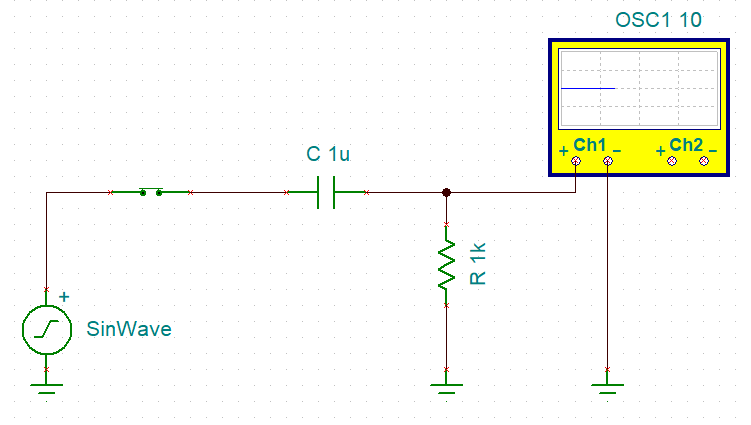
\includegraphics[width=0.85\columnwidth]{circuit_ex7.png}
			\caption{\label{fig:ex7Circuit}The circuit diagram created in TINA to measure the amplitude and phase response of an RC circuit.}
		\end{figure}
		\subsection{Results \& Analysis}
		The amplitude and phase data simulated by TINA was plotted in figure \ref{fig:ex7Results} along with the data measured from the physical circuit. It is clear that the data matches within the bounds of uncertainty. The uncertainty for these measurements were made either from the measuring limitations of the oscilloscope (i.e. the amount of decimals displayed) or where the measurement was not constant - such as in cases of low frequency ($<10 \,\text{Hz}$) - the average and standard deviation of 10 measurements was taken.\\
		
		These simulation curves displayed, and hence the data, match that described by equations \ref{eq:amplitude} and \ref{eq:phase}. We see that the circuit behaves at a high pass filter with negative gain for frequencies lower than $1 \,\text{kHz}$. The output is out of phase for these lower frequencies and results in destructive interference.
		
		\begin{figure}
			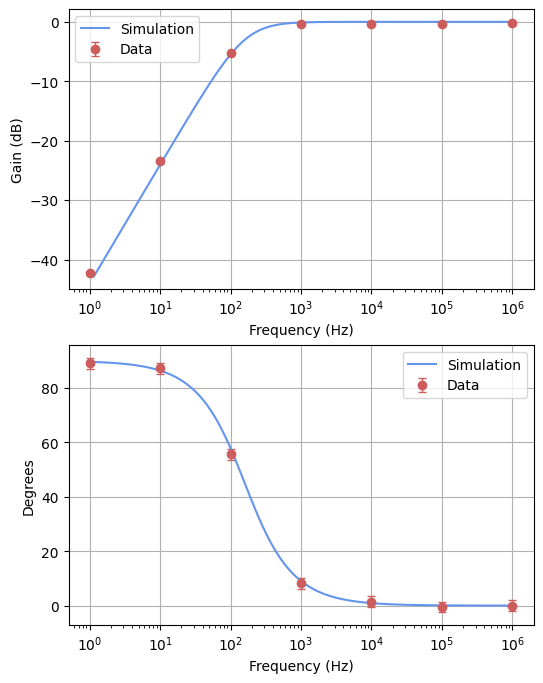
\includegraphics[width=0.85\columnwidth]{ex7_dualPlot.png}
			\caption{\label{fig:ex7Results}Bode plot of exercise 7. The circuit is a high pass filter with $R = 1 \text{k}\Omega$, $C = 1 \mu\text{F}$. Note that errorbars are included on both graphs however in some cases are to small to see.}
		\end{figure}
		
	\section{Exercise 12: Diodes}
		\subsection{Theory}
		The aim of exercise 12 is determine the I-V curve for a diode in forward and reverse bias. A diode is a PN junction which is either in forward bias or reverse bias depending on the direction of current flow across it, see figure \ref{fig:pnJunction} \cite{manual}. When forward biased the voltage source is connected such that the anode is positive compared to the cathode, current will flow. When reverse biased, the voltage source is opposite in polarity with respect to forward bias. The cathode has a positive voltage compared to the anode. Due to the nature of PN junctions no current will flow up to a breakdown voltage \cite{manual}.
		
		\begin{figure}
			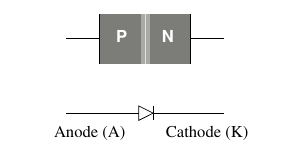
\includegraphics[width=0.85\columnwidth]{pnJunction.png}
			\caption{\label{fig:pnJunction}Above: the PN junction of the diode. Below: the schematic symbol of the diode \cite{manual}.}
		\end{figure}
		
		\subsection{Methodology}
		
		The aim of this exercise was to measure the I-V curve for the 1N1418 diode. A circuit was designed in TINA to do this using a resistor to limit the current flow and a voltage source to vary to vary the input voltage, see figure \ref{fig:ex12Circuit}. A multimeter was used to measure the current. A $470 \,\Omega$ resistor was chosen to limit the current flow. The voltage was varied between $-10 \,\text{V}$ and $10 \,\text{V}$ and recorded and plotted in figure \ref{fig:IVCurveLinear}.\\
		
		The circuit was then driven with a AC sin wave with frequency $500 \,\text{Hz}$ and peak-to-peak amplitude of $3\,\text{V}$. The voltage drop across the resistor was measured by subtracting oscilloscope measurements of the voltage before and after the resistor. This oscilloscope data was recorded and plotted in figure \ref{fig:ex12bResults}. A $10 \,\mu\text{F}$ capacitor was added in parallel across the resistor and the measurement was repeated. This was recorded and plotted in figure \ref{fig:ex12bResultsWithCap}.
		
		\begin{figure}
			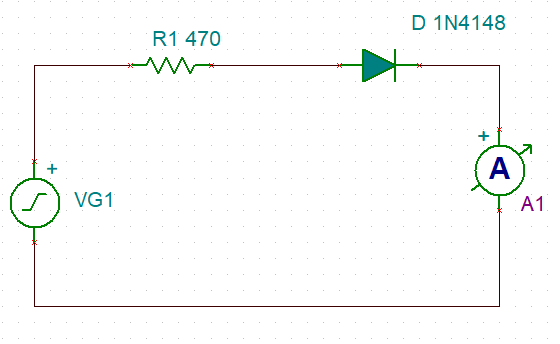
\includegraphics[width=0.85\columnwidth]{ex12Circuit.png}
			\caption{\label{fig:ex12Circuit}Circuit diagram create in TINA for exercise 12. Note that this doesn't include the capacitor added in the second half of the exercise.}
		\end{figure}
	
		\subsection{Results \& Analysis}
		From figure \ref{fig:IVCurveLinear} we can see the linear proportionality of current to voltage as depicted by Ohm's law when in forward bias. In reverse bias we see no current as the breakdown voltage of the diode was much higher than the maximum output of the voltage generator and hence any leak-through current was too small to be measured by the multimeter. According to a manufacturer data-sheet \cite{diodeData}, the 1N4148 diode needs a reverse bias voltage of $\approx 75 \,\text{V}$ before it leaks a current on the order of micro-amps.\\
		
		When driven with the sin wave, we see no voltage across the resistor when the AC signal is in reverse bias, and a peak when the signal is in forward bias. This is again expected and due to the diode stopping current flow in reverse bias. When the capacitor is added, we see a similar effect but with some distinct differences. The capacitor in parallel causes less current to flow across the resistor making for a smaller peak voltage drop across it, this can be visually seen. We also see a delay in the peak voltage drop across the resistor, and a sustained voltage drop even during reverse bias. This is due to the nature of the capacitor taking time to charge and discharge. We see the peak voltage drop lag behind as the capacitor charges and we see a decaying voltage drop in reverse bias as the capacitor discharges.
		
		\begin{figure}
			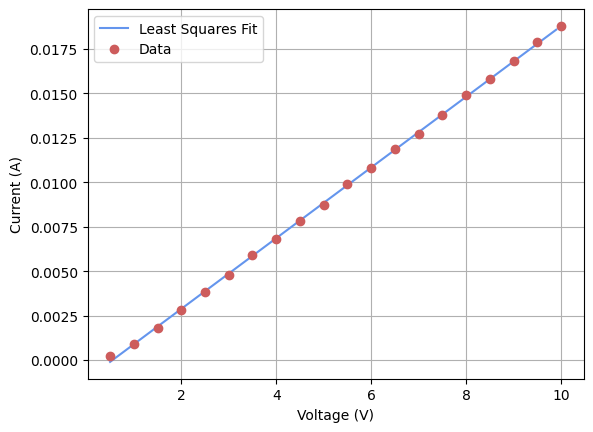
\includegraphics[width=0.85\columnwidth]{IVCurveLinear.png}
			\caption{\label{fig:IVCurveLinear}I-V curve for the circuit in forward and reverse bias. As the breakdown voltage of the diode was much higher than the maximum output of the voltage generator and hence any leak-through current was too small to be measured by the multimeter.}
		\end{figure}
	
		\begin{figure}
			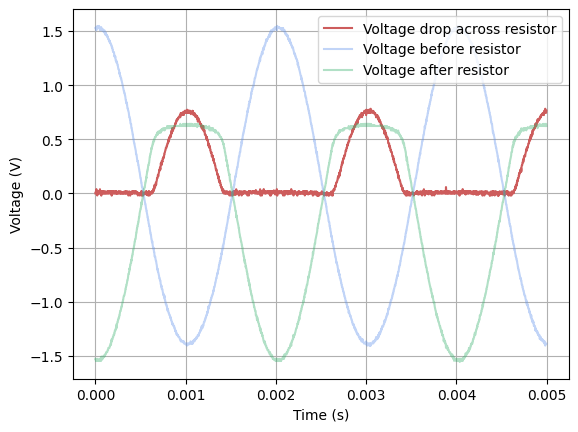
\includegraphics[width=0.85\columnwidth]{ex12bResults.png}
			\caption{\label{fig:ex12bResults}Voltage drop over the resistor when the circuit from exercise 12 was driven by a sin wave.}
		\end{figure}
	
		\begin{figure}
			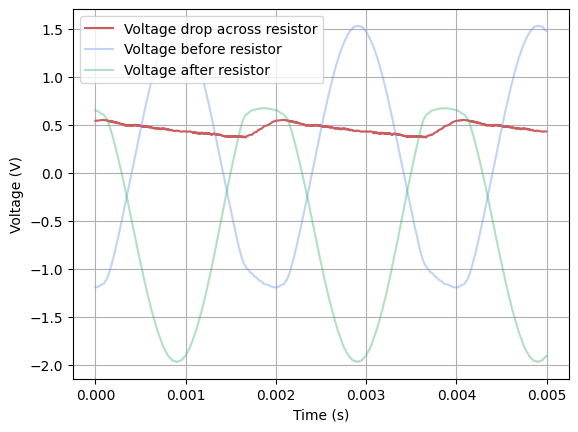
\includegraphics[width=0.85\columnwidth]{ex12bResultsWithCap.png}
			\caption{\label{fig:ex12bResultsWithCap}Voltage drop over the resistor with a capacitor in parallel, when the circuit from exercise 12 was driven by a sin wave.}
		\end{figure}
		
	\section{Exercise 19: Transistors as a Current Amplifier}
		\subsection{Theory}
		A transistor is a 3 terminal semiconductor device comprised of the joining of two PN junctions. They can be arranged in two layouts, npn or pnp, see figure \ref{fig:transistors} \cite{horowitz}. In this exercise, a transistor is used as an amplifier. A small current $I_B$ must flow into the base to allow current $I_C$ to flow through the detector. The current gain - the ratio between these two currents - is determined by the following equation \cite{horowitz}.
		\begin{equation}
			\beta = {I_C \over I_B}
			\label{eq:currentGain}
		\end{equation}
		
		\begin{figure}
			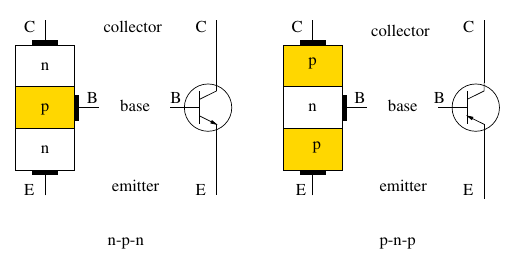
\includegraphics[width=0.85\columnwidth]{transistors.png}
			\caption{\label{fig:transistors}A diagram of the two layouts of transistors \cite{manual}.}
		\end{figure}
		
		\subsection{Methodology}
		
		This exercise aims to simulate a current amplifying circuit and calculate the current gain for a 2N4400 transistor. The circuit was designed and simulated in TINA, see figure \ref{fig:currentAmplifier}. The resistor values were chosen as given by the lab manual \cite{manual}, with their purpose being to reduce the current flow into the base of the transistor. The TINA software's DC analysis was used to measure the current from the ammeters. These currents were recorded and then equation \ref{eq:currentGain} was used to calculate the current gain based on the current running through the collector and the base.
		
		\begin{figure}
			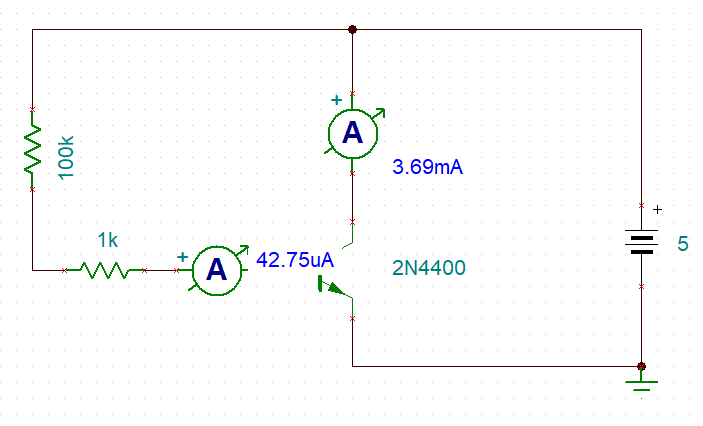
\includegraphics[width=0.85\columnwidth]{circuitOn.png}
			\caption{\label{fig:currentAmplifier}The circuit setup in TINA to demonstrate current amplification with transistors.}
		\end{figure}
		
		\subsection{Results \& Analysis}
		Equation \ref{eq:currentGain} was used to calculate the current gain of the circuit using the data from figure \ref{fig:currentAmplifier}. With a base current of $42.75 \,\mu\text{A}$ and a collector current of $3.69 \,\text{mA}$, the current gain, $\beta$, was calculated to be $\beta = 86.32$.
	
	\section{Exercise 20: Transistors as a Switch}
		\subsection{Theory}
		Another applications of transistors is as a switch. Make for good switches as they are small, cheap, reliable, and can switch rapidly \cite{manual}. Similarly to how the current amplifier required a current (and hence voltage) through the base to allow current to flow through the collector, if we think of the path from the collector to the emitter as the primary path, then the voltage at the base controls if the current can flow through this path. The "switch" is on if there is sufficient voltage at the base (approx. $0.7 \,\text{V}$), and off where there isn't.\\
		
		The aim this exercise is the vary the load resistance and look at the effect it has on the switching action. The load resistor is placed in series with the collector of the transistor. The output voltage from a sample circuit (figure \ref{fig:ex20Circuit}) is expected to look as shown in figure \ref{fig:loadResistorDiagram}. This graph is split up into three distinct sections. In section A the transistor switch is off, there is no current flowing from the collector and hence the output is 6 V. In section B, the transistor switch is partially on, as the current increases, the voltage across the load resistor increases and the output drops. In section C, the transistor is fully on and said to be saturated \cite{manual}.
		
		
		\begin{figure}
			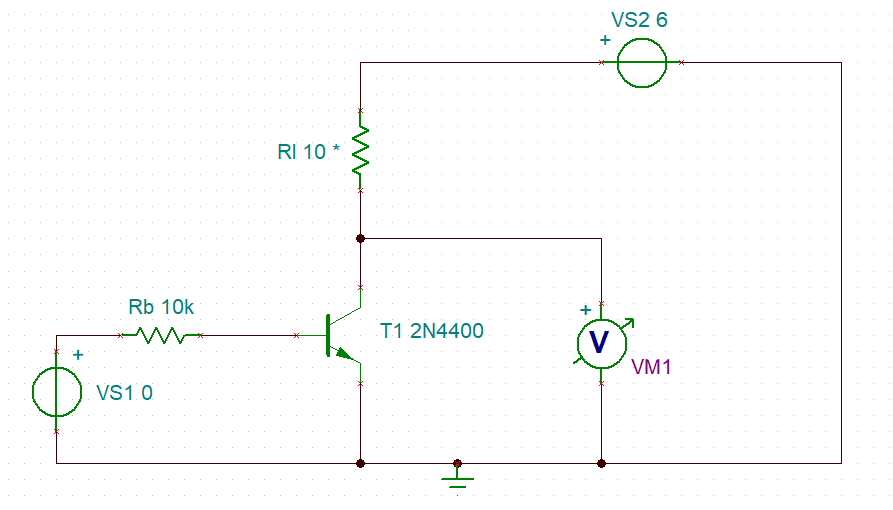
\includegraphics[width=0.85\columnwidth]{ex20Circuit.png}
			\caption{\label{fig:ex20Circuit}The circuit diagram for exercise 20, created in TINA. The load resistor, $Rl$, was setup so that it could be varied.}
		\end{figure}
		\begin{figure}
			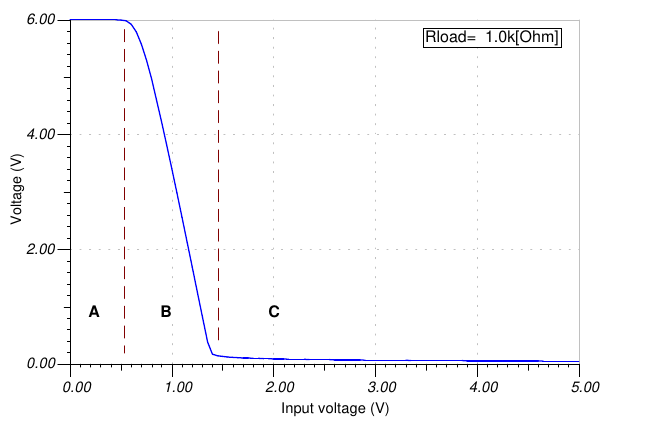
\includegraphics[width=0.85\columnwidth]{loadResistorDiagram.png}
			\caption{\label{fig:loadResistorDiagram}A diagram of the voltage response with a load resistor of resistance $1 \,\text{k}\Omega$ \cite{manual}.}
		\end{figure}
		
		
		\subsection{Methodology}
		
		The circuit was constructed in TINA as directed by the exercise \cite{manual}, see figure \ref{fig:ex20Circuit}. The load resistor was set up as a control target in TINA to vary its resistance during analysis. The voltage response for load resistances of $10\,\Omega$, $100\,\Omega$, $1\,\text{k}\Omega$, and $10\,\text{k}\Omega$ were simulated and recorded in figure \ref{fig:ex20Results}.
		
		\subsection{Results \& Analysis}
		
		Each voltage response simulation for each load resistor was recorded and plotted in figure \ref{fig:ex20Results}. We see that the results match that of what is expected in figure \ref{fig:loadResistorDiagram}. We see that the slope of the B section of the voltage response depends on the load resistance with a higher resistance yielding a sharper slope. The lower load resistances of $10\,\Omega$ and $100\,\Omega$ never reach saturation for an input voltage less than the voltage before the load resistor.
		
		\begin{figure}
			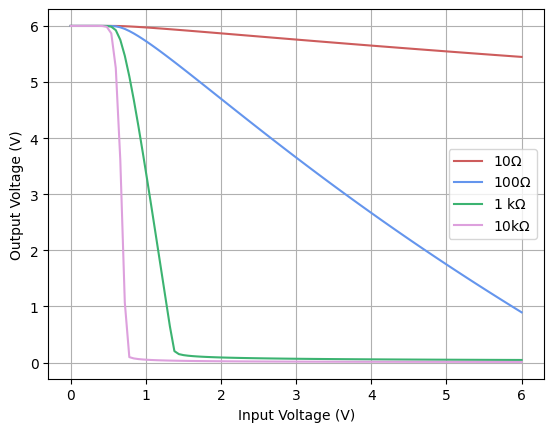
\includegraphics[width=0.85\columnwidth]{ex20Results}
			\caption{\label{fig:ex20Results}The results from exercise 20. We see that the lower load resistances never reach saturation.}
		\end{figure}
		
	\section{Exercise 21: LDR controlled switch}
		\subsection{Theory}
		In this exercise, an LDR is used in a voltage divider to control the voltage at the base of the transistor. The aim was to create an LED alarm which would light up if in darkness but be off in brightness. The LDR changes resistance based on the level of light with its highest resistance in darkness. This will change the voltage at the base of the transistor as determined by the voltage divider equation \cite{seeed}:
		\begin{equation}
			V_\text{out} = V_\text{in} \frac{R_2}{R_1 + R_2}
			\label{eq:voltageDivider}
		\end{equation}where $V_\text{out}$ is the potential before the pair of resistors $R_1$ and $R_2$, $V_\text{in}$ is the potential between the resistors.
		
		\subsection{Methodology}
		The circuit was first designed in TINA as shown in figure \ref{fig:ex21Circuit}. Here the resistors labelled R and LDR make the voltage divider. Note that the LDR here is represented as a resistor for simplicity of simulation. With reference to the voltage divider, equation \ref{eq:voltageDivider}, $R_1$ is the resistor labelled R, and $R_2$ is the lDR. The component values for this circuit were determined analytically. First the circuit was split into two loops: one containing the battery, LED, load resistor, and the collector and emitter of the transistor. The other containing the battery, $R_1$ and the LDR.\\
		
		The first loop was considered such that the current flowing through was sufficient to light the LED. The load resistance was chosen to set this current, based on the voltage after the LED, calculated using the reverse-bias voltage of the LED. The manual recommends a current of $5 \,\text{mA}$ and hence using Ohm's law, the resistor was determined to ideally be $640\,\Omega$. As the resistors available to use were a limited selection, a $680 \,\Omega$ resistor was used instead. The second loop was considered to have greater than $0.7\,\text{V}$ at the base of the transistor when the LDR had high resistance and less than $0.7\,\text{V}$ when the LDR had low resistance. The LDR was measured in complete darkness and in the light of the room to find its resistance at these levels of brightness. The voltage divider equation was then used to determine that $R_1 = 10\,\Omega$ would provide sufficient voltage at the base. A small resistor $R_b$ at the base terminal of the transistor was used to limit the current through the transistor. A value of $1\,\Omega$ was chosen. The circuit was then simulated to check if the values chosen were correct before it was constructed. The circuit was constructed and it was determined visually if the circuit worked as expected.
		
		\begin{figure}
			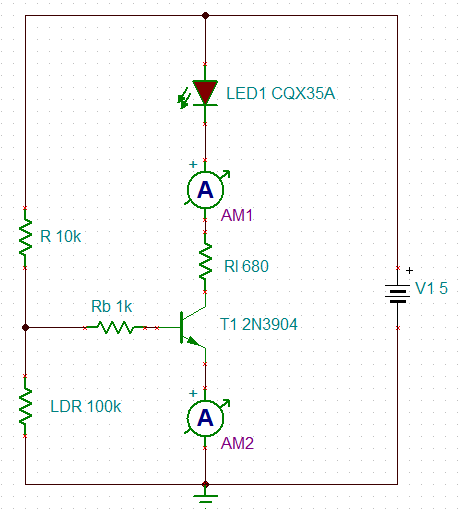
\includegraphics[width=0.85\columnwidth]{ex21Circuit.png}
			\caption{\label{fig:ex21Circuit}Circuit diagram for exercise 21 as designed in TINA. Here the LDR is represented as a 100k resistor to emulate it being in darkness.}
		\end{figure}
		
		\subsection{Results \& Analysis}
		The LDR was measured to have a $\approx1\,\text{k}\Omega$ resistance in the light of the room and $\approx100\,\text{k}\Omega$ in darkness. The circuit was constructed and behaved as expected. In figure \ref{fig:ex21Off}, we see the circuit in the light of the room, the LED is off. In figure \ref{fig:ex21On}, we see the circuit with the LDR covered, the LED is on and hence the circuit works as expected.\\
		
		The average yearly cost of this circuit was calculated. The power requirement of the circuit was calculated to be $2.25\,\text{mW}$ when the LED was off, and $25.75\,\text{mW}$ when the LED was on. Assuming an average of 12 hours of brightness and 12 hours of darkness in each day and a unit cost (cost per kWh) to be 0.18 euro, the yearly cost of the circuit was determined to be 2.21 cent. See appendix 1 for the full calculation.
		
		\begin{figure}
			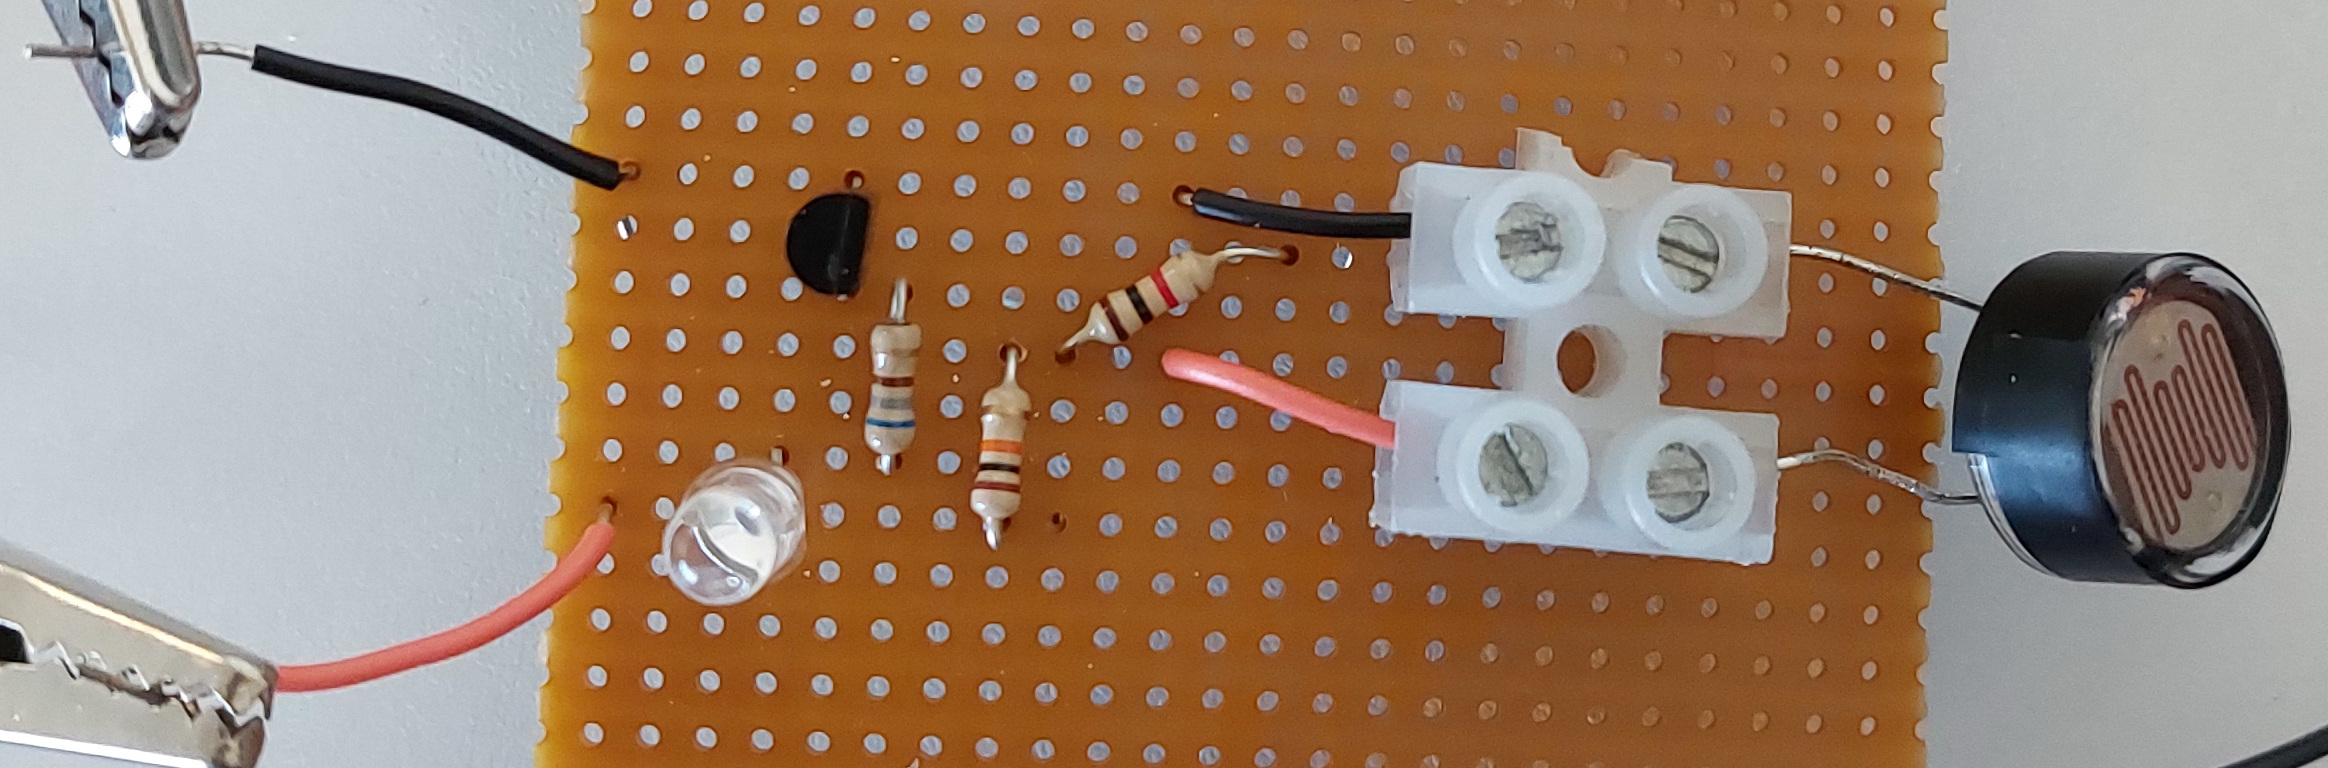
\includegraphics[width=0.85\columnwidth]{ex21Off.jpg}
			\caption{\label{fig:ex21Off}A picture of the circuit from exercise 21. The circuit is powered but the LED is off as the LDR is receiving light.}
		\end{figure}
		\begin{figure}
			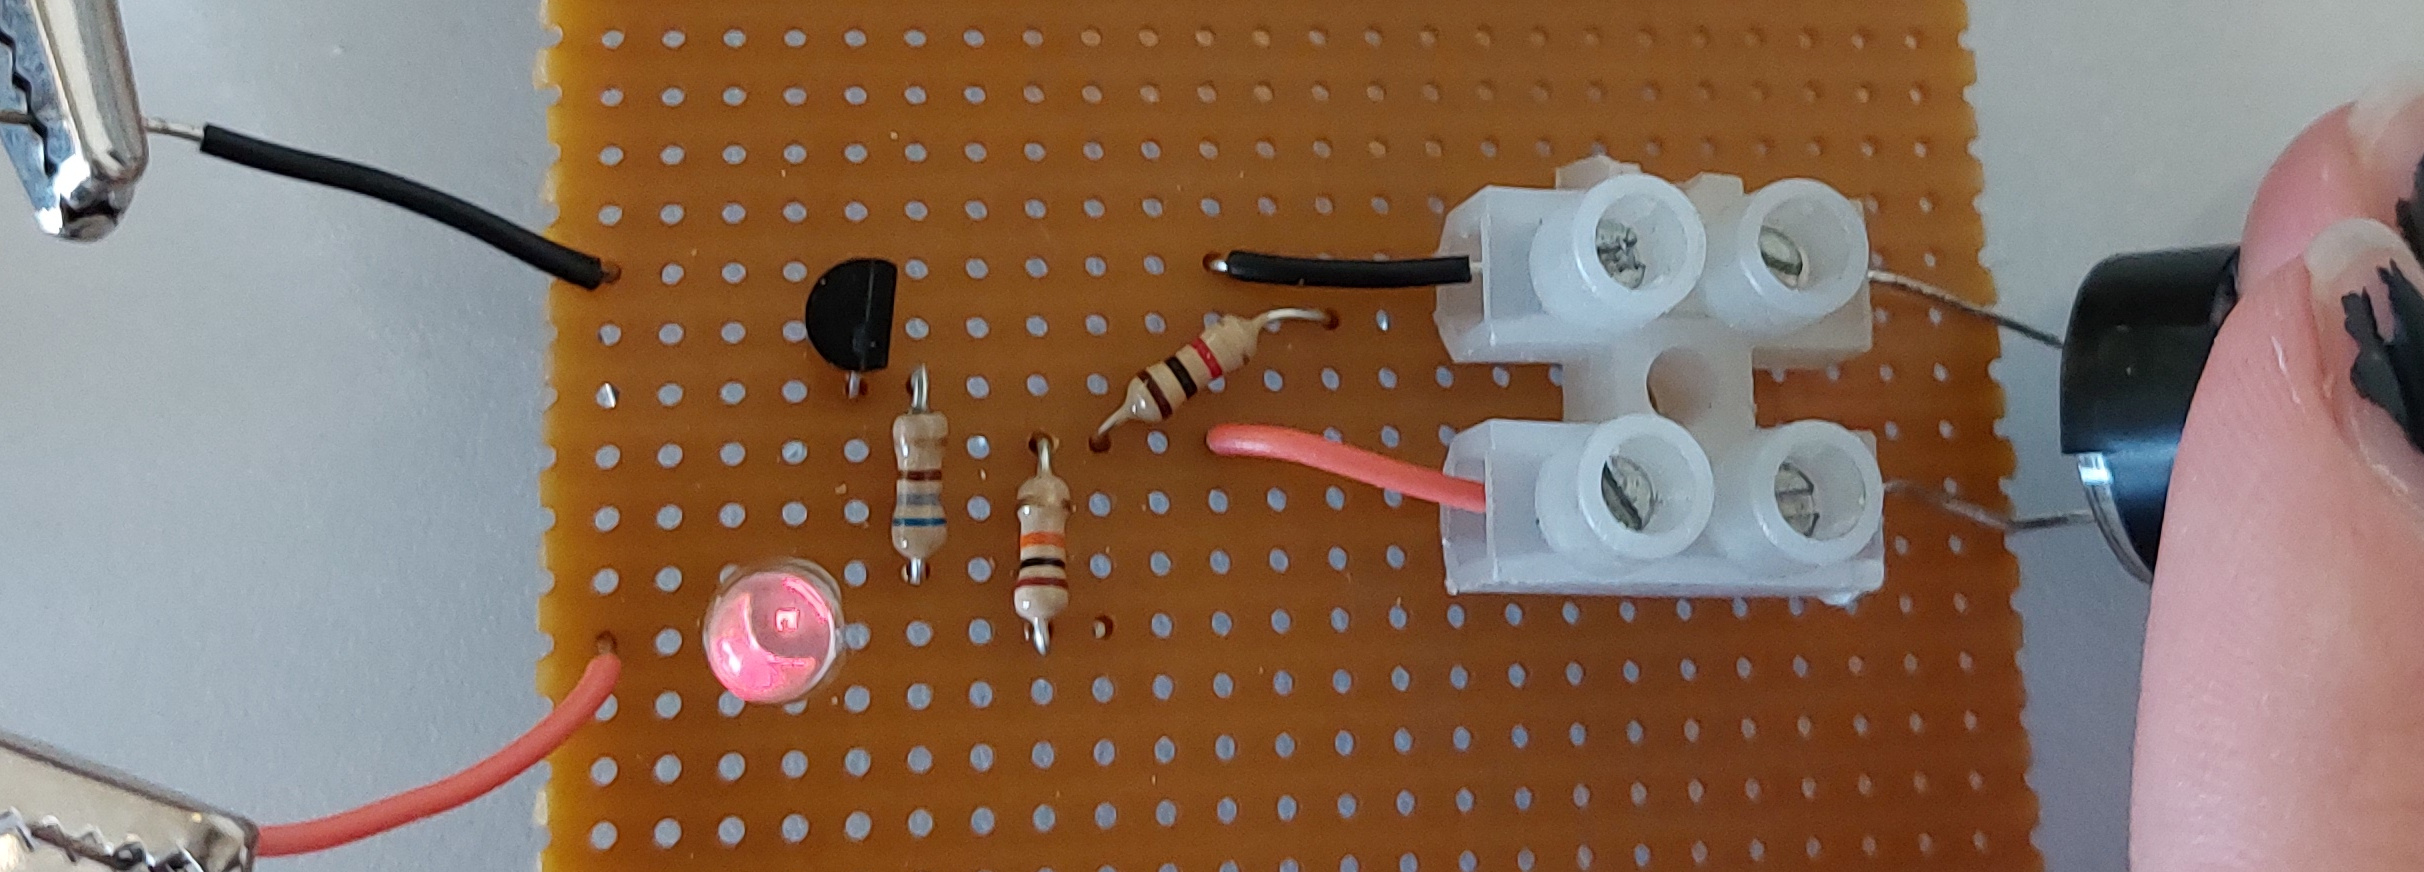
\includegraphics[width=0.85\columnwidth]{ex21On.jpg}
			\caption{\label{fig:ex21On}A picture of the circuit from exercise 21. The circuit is powered and the LED is on as the LDR is covered and not receiving light.}
		\end{figure}
		
	\section{Exercise 25: Non-Inverting Amplifier}
		\subsection{Theory}
		An Op-Amp (Operational Amplifier) is a integrated circuit device which can make it easier to construct amplifiers or other systems in circuits \cite{manual}. An Op-Amp has two input terminals and acts as a differential amplifier, amplifying the difference between the inputs by a constant gain.\\
		
		Negative feedback is when a portion of amplified output signal is fed back into the inverting input \cite{horowitz}. An Op-Amp with negative feedback can be described by two rules \cite{manual}: 1. The output tries to to make the voltage difference between the inputs zero. 2. The inputs draw no current. Negative feedback can be used to allow the gain of the amplifier to be controlled by the feedback network \cite{manual}. The gain of the circuit is the ratio between the output and input signals. It can be calculated in decibels by the following relation \cite{sengpiel}:
		\begin{equation}
			L_V = 20 \log_{10}\left(\frac{V}{V_0}\right)\,\text{dB}
			\label{eq:gain}
		\end{equation}where $V$ is the output voltage and $V_0$ is the input voltage. The ratio of the voltages can also be determined by the feedback network resistors, as derived in section 5.5 of the manual \cite{manual}:
		\begin{equation}
			\frac{V_\text{out}}{V_\text{in}} = 1 + \frac{R_f}{R_i}
			\label{eq:resistorRatio}
		\end{equation}where $R_f$ and $R_i$ are the resistors in the feedback loop labelled in figure \ref{fig:ex25Circuit}.
		
		\subsection{Methodology}
		A simple amplifying Op-Amp circuit was constructed following the diagram from the manual \cite{manual}, see figure \ref{fig:ex25Circuit}. Components were chosen such to obtain a gain of 20 dB. Using equation \ref{eq:gain} a voltage ratio of $\frac{V}{V_0} = 10 = 1 + \frac{R_f}{R_i}$ was determined and subsequently suitable resistors could be chosen to satisfy equation \ref{eq:resistorRatio}. As the ratio of $\frac{R_f}{R_i} = 9$ is impractical, a ratio of $\frac{R_f}{R_i} = 10$ was used to match the components available. Resistors $R_f = 47\,\text{k}\Omega$ and $R_i = 4.7\,\text{k}\Omega$ were used. The circuit was driven by a $1\,\text{kHz}$ sine wave which was recorded using an oscilloscope along with the output. A $1 \,\mu \text{F}$ capacitor was then inserted across $R_f$ and the measurement was repeated.
		
		\begin{figure}
			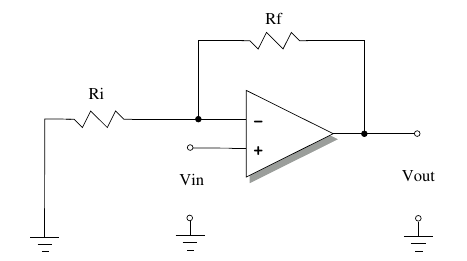
\includegraphics[width=0.85\columnwidth]{ex25Circuit.png}
			\caption{\label{fig:ex25Circuit}The circuit diagram provided by the manual for exercise 25 \cite{manual}.}
		\end{figure}
	
		\subsection{Results \& Analysis}
		The results measured from the oscilloscope were recorded in table \ref{tab:ex25Results} and \ref{tab:ex25ResultsWithCapacitor} and the gain was plotted against frequency in figures \ref{fig:ex25Results} and \ref{fig:ex25ResultsWithCapacitor} for the circuit without and with the capacitor respectively. This calculation was done using equation \ref{eq:gain}.\\
		
		For the circuit without the capacitor we see a constant gain up to a specific frequency where the gain attenuates, this frequency was $10^4\,\text{Hz}$. Note although the exercise asked for a gain of $20\,\text{dB}$, the gain here is higher. This is due to the altering of the ratio as mentioned in the theory section to accommodate for the components available to use.\\
		
		For the circuit with the capacitor we see the same shape but with a reduced bandwidth. This is because of the inverse frequency dependence of the impedance of a capacitor as described by equation \ref{eq:capacitor}. As the frequency increases, the voltage at the inverting input approaches that of the non-inverting input and the gain hence goes to zero.
		
		\begin{table}[]
			\resizebox{0.5\columnwidth}{!}{%
				\begin{tabular}{@{}ll@{}}
					\toprule
					Frequency (Hz) & Output (V) \\ \midrule
					10             & 5.43       \\
					100            & 5.43       \\
					1000           & 5.43       \\
					10000          & 5.41       \\
					12000          & 3.10       \\
					15000          & 2.37       \\
					20000          & 1.56       \\
					25000          & 1.01       \\
					30000          & 0.680      \\ \bottomrule
				\end{tabular}%
			}
			\caption{The data measured using the oscilloscope for exercise 25.}
			\label{tab:ex25Results}
		\end{table}
	
		\begin{table}[]
			\resizebox{0.5\columnwidth}{!}{%
				\begin{tabular}{@{}ll@{}}
					\toprule
					Frequency (Hz) & Output (V) \\ \midrule
					10             & 1.361      \\
					12             & 1.36       \\
					14             & 1.32       \\
					16             & 1.27       \\
					18             & 1.21       \\
					20             & 1.11       \\
					25             & 0.9         \\
					30             & 0.8         \\
					40             & 0.7         \\
					50             & 0.63        \\
					70             & 0.57        \\
					100            & 0.527       \\
					200            & 0.52        \\
					500            & 0.51        \\
					1000           & 0.5         \\
					5000           & 0.5         \\
					10000          & 0.5         \\
					25000          & 0.5         \\
					43000          & 0.5         \\ \bottomrule
				\end{tabular}%
			}
			\caption{The data measured using the oscilloscope for exercise 25 with the inclusion of the $1\,\mu\text{F}$ capacitor.}
			\label{tab:ex25ResultsWithCapacitor}
		\end{table}
		
		\begin{figure}
			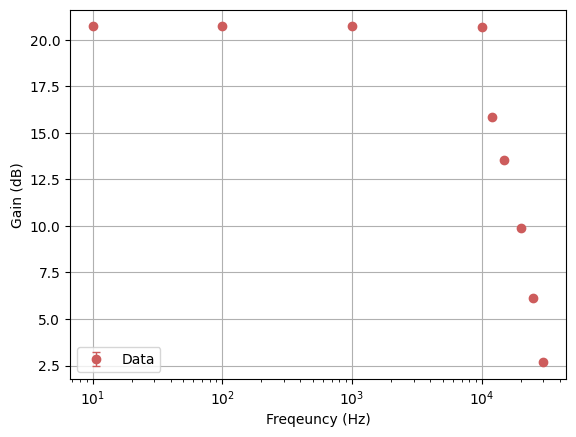
\includegraphics[width=0.85\columnwidth]{ex25Results.png}
			\caption{\label{fig:ex25Results}Data from the measurements of exercise 25. We see a constant gain until the attenuation frequency.}
		\end{figure}
		
		\begin{figure}
			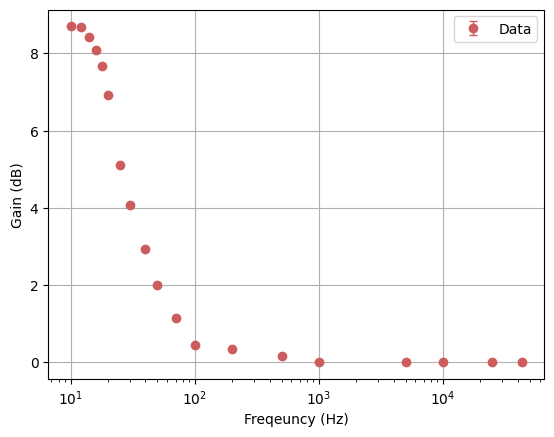
\includegraphics[width=0.85\columnwidth]{ex25ResultsWithCapacitor.png}
			\caption{\label{fig:ex25ResultsWithCapacitor}Data from the measurements of exercise 25 with the insertion of the capacitor. We see a smaller bandwidth.}
		\end{figure}
		
	\section{Exercise 27: Digital-to-Analogue Converter}
		\subsection{Theory}
		A Digital-to-Analogue Converter, or DAC, is a circuit which takes a digital signal such as a binary number and converts it to an analogue voltage. In a 4-bit DAC, a four digit binary number is used to represent a signal (i.e. 1011). The DAC circuit will then output a voltage corresponding to the input signal. A common DAC circuit uses a summing amplifier to sum the currents from input branches corresponding to the signal, see figure \ref{fig:summingAmp}. The output voltage is a combination of each of the input voltages weighted by their corresponding resistor. The output voltage is given by the following equation \cite{manual}:
		\begin{equation}
			V_\text{out} = -R_f \left(\frac{V_1}{R_1} + \frac{V_2}{R_2} + \dots + \frac{V_N}{R_N}\right)
			\label{eq:DAC}
		\end{equation}
		
		\begin{figure}
			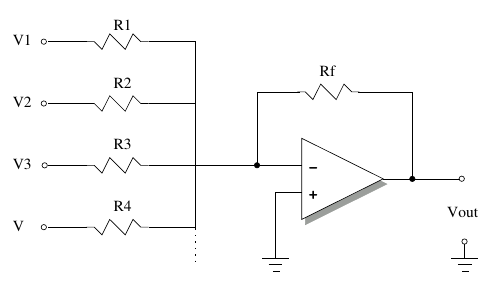
\includegraphics[width=0.85\columnwidth]{summingAmp.png}
			\caption{\label{fig:summingAmp}A sample summing amplifier use to make DAC circuits \cite{manual}.} 
		\end{figure}
		
		\subsection{Methodology}
		A DAC circuit was constructed in TINA following the sample summing amplifier in figure \ref{fig:summingAmp}. A 4-bit signal was used as the input with a digital voltage high of $5 \,\text{V}$ and a low of $0 \,\text{V}$. Switches were used to manually select the input signal. From the binary number 0000 to 1111 there are 16 numbers inclusive. Each of these was mapped to a voltage with $0000 \to 0 \,\text{V}$ and $1111 \to -3 \,\text{V}$ and the rest were spaced evenly between. Equation \ref{eq:DAC} was then used to determine the input resistance needed to achieve these results. Using the input signals which isolated one resistor (i.e. 0001, 0010, 0100, and 1000), a ratio between each input resistor and $R_f$ could be determined. $R_f$ was then arbitrarily picked and the input resistors were calculated based on these ratios.
		
		\subsection{Results \& Analysis}
		The circuit diagram as constructed in TINA is shown in figure \ref{fig:ex27ResultsOff} with an input of $0000$, and in figure \ref{fig:ex27ResultsOn} with an input of $1111$. It can clearly be seen that resistances chosen map the DAC accordingly. Note that an ideal Op-Amp was used in this instance.
		
		\begin{figure*}
			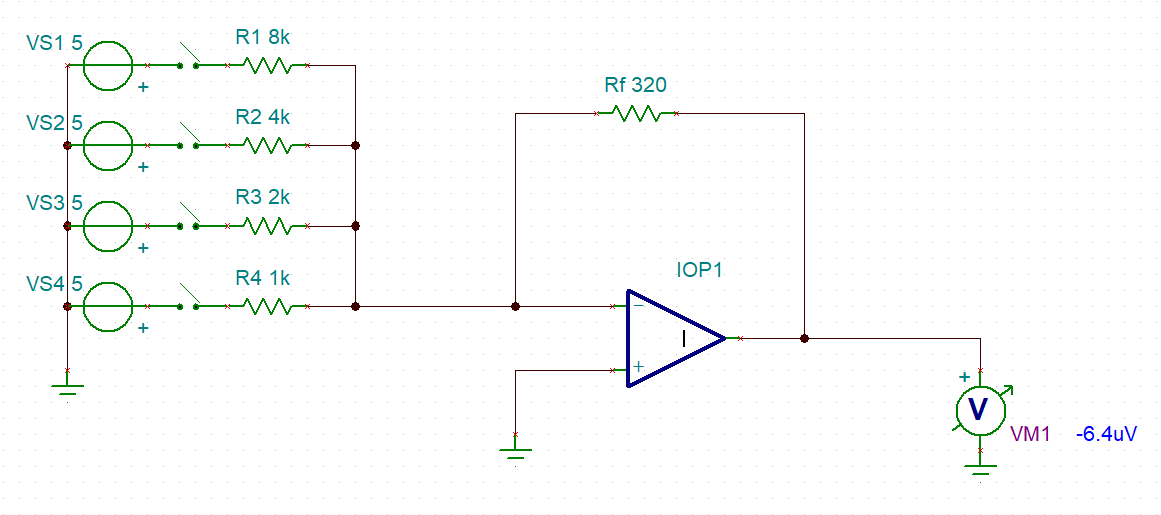
\includegraphics[width=1.6\columnwidth]{circuitZero.png}
			\caption{\label{fig:ex27ResultsOff}}
		\end{figure*}
		\begin{figure*}
			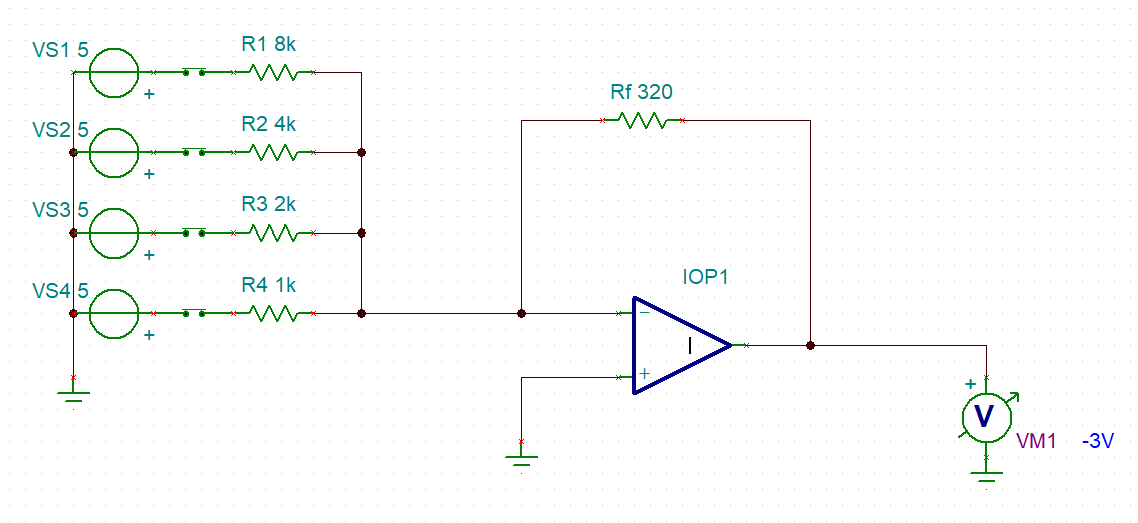
\includegraphics[width=1.6\columnwidth]{circuitMax.png}
			\caption{\label{fig:ex27ResultsOn}}
		\end{figure*}
		
	\clearpage
	\bibliography{electronics.bib}% Produces the bibliography via BibTeX.
	
	\clearpage
	\onecolumngrid
	\appendix
	\section{Circuit cost calculation for exercise 21}
	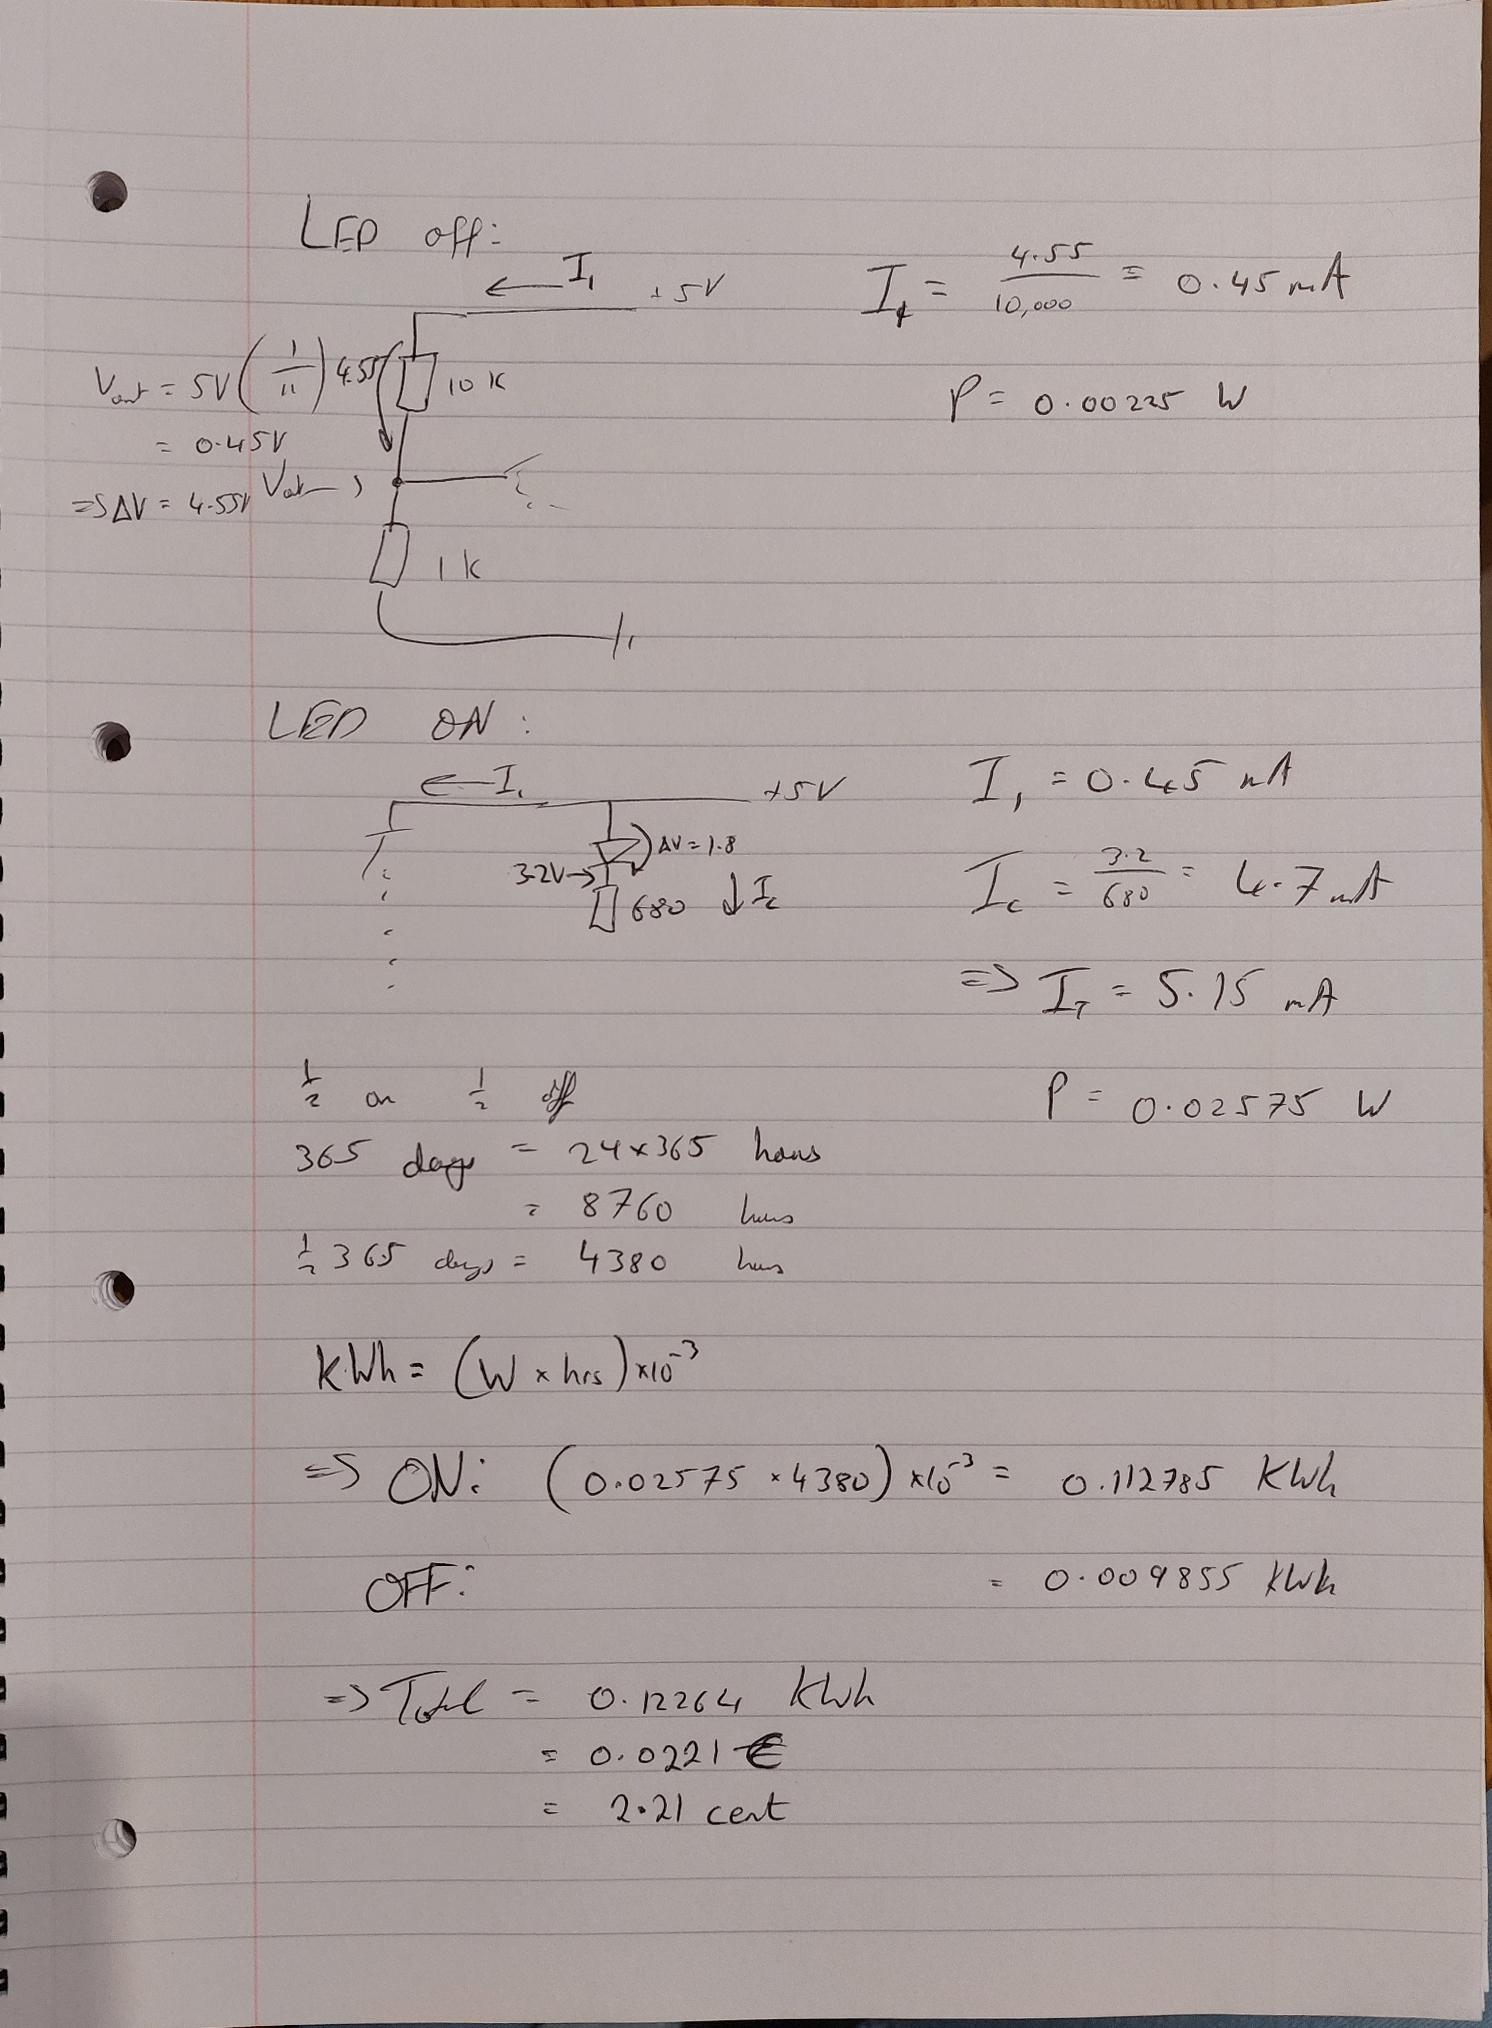
\includegraphics[width=\linewidth]{ex21_calc.jpg}

	
	
\end{document}

